\subsection{Predstavitev stroja in kosa}
Za svoj stroj sem si izbral dolgo-stružni avtomat Gauthier GM-127
prikazan na sliki \ref{gauthier_priblizano}.
Ima 5 držal za orodja in 3 gnana orodja, vidnih na spodnji
sliki \ref{gauthier_priblizano}. Omogoča struženje do ø12.7 mm.
Ima tudi možnost nadgradnje z roko za preprijem kosa pri odrezovanju in
povrtavanje ali vrezovanje navoja iz druge strani.

\begin{figure}[H]
	\begin{center}
		\includegraphics[width=8cm]{gauthier_slika.jpg}
		\caption{Krivuljni avtomat Gauthier GM-127, katerega sem nastavljal
			\cite{interna}}
		\label{gauthier_priblizano}
	\end{center}
\end{figure}

Za izdelek, sem si izbral pušo iz materjala 1.4305.
Na sliki \ref{delavniska_risba} je delavniška risba z
merami in tolerancami kosa. Stranki je najbolj pomembna dolžina
kosa 6.8 \(\pm\) 0.05 mm, zato se ta kasneje posebej preverja z
100 \% kontrolo. Pomemben je tudi premer izvrtine \(\phi\) 1.4 \(+\) 0.1 mm.
Premer puše \(\phi\) 5 \(\pm\) mm je tudi pomemben, ampak se ga
ne posebej preverja, saj je odvisen od materiala, ki je dobavljen.
Dimenzije posnetij niso pomembne, saj jih je tudi težko izmeriti,
pomembno je le, da robi niso ostri in da nimajo srha.

\begin{figure}[H]
	\begin{center}
		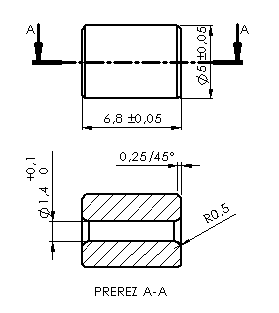
\includegraphics[width=8cm]{izdelek_risba.png}
		\caption{Risba končnika žice
			\cite{interna}}
		\label{delavniska_risba}
	\end{center}
\end{figure}

Izdelek se uporablja kot končnik žice, katera se napelje skozi
luknjo v sredini izdelka. Za lažjo napeljavo, so v luknji zahtevana
posnetja v obliki radiusa. Za tem se končnik fiksira z
stiskanjem v hidravlični stiskalnici.